\section{Putting it altogether: building and training a CNN on graphs}

In order to test our understanding of the algorithms and to gain intuition about the potential of GCNN on classic Neural Network tasks, we have implemented the different algorithms presented in the paper. When coming to Neural Networks, two experiments allow to rapidly gain intuition about the potential of an architecture:
\begin{itemize}
    \item Classification: Check that the architecture proposed is able to classify a simple data-set with acceptable performance.
    \item AutoEncoders : Construct an encoder-decoder architecture to verify that the model allows to construct interesting embedded representation of simple data. 
\end{itemize}

Following the work of the authors, we decided to implement both experiments using a classic dataset: the MNIST dataset of handwritten digits \cite{lecun1998mnist}. This dataset has multiples advantages: it is reasonable in size, it is a widely used benchmark on which a vast majority of algorithms have been tested, and it uses images which helps to rapidly debug implementation (we can basically plot and check everything). Still, using MNIST has a few downsides we would like the reader to be aware of: the samples are highly pre processed (centered, resized, and upright), which makes it easier to classify, and more specifically to our case, images are not the best examples of signals defined over \emph{arbitrary} structures (like data over sensing networks). 

\subsection{A classic benchmark: The MNIST classifier}
To implement a full GCNN classifier over the MNIST dataset, we took the approach to implement it in two times. First, we implemented a slow but easier to debug program using equation \ref{eq:localized_filter} for filtering, and Transition matrix based Max Pooling. For this first implementation, we have tried different approaches based on the classic LeNet5 architecture \cite{LeCun1998-Lenet5}, to finally come up with our best working one. Our basic Graph Convolutional stack is hence composed of the following operations:
\begin{itemize}
    \item Perform a Graphical filtering with largest Laplacian power $K_i=5$, and number of filters $n_i=5$.
    \item Perform a ReLu Non-Linearity
    \item Perform 2 Max Pooling to reduce the overall size about a factor $\sim 4$
\end{itemize}

Note that we chose to apply every filter to every feature independently, which means that the last feature map will have a depth equal to $\prod_i n_i$. 

Our first general architecture is then a combination of two such Graph Convolutional stacks, followed by 2 fully connected layers and a softmax output layer, as represented on figure \ref{fig:mnist_classifier}. 

\begin{figure}
    \centering
    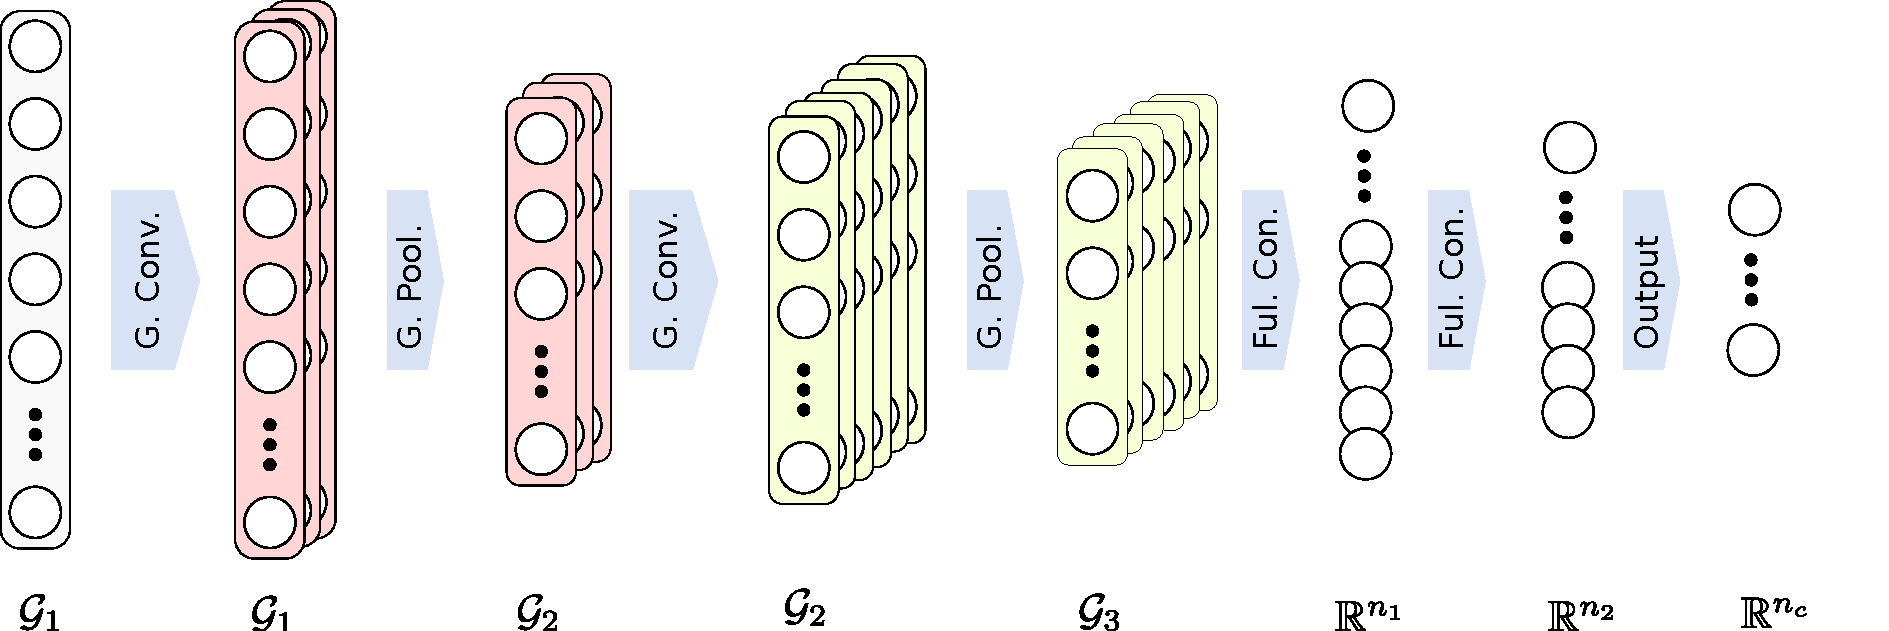
\includegraphics[width=\textwidth]{img/classifier.pdf}
    \caption{The architecture used to classify MNIST, with signal structure }
    \label{fig:mnist_classifier}
\end{figure}

We trained this architecture using a classic regularized cross entropy loss:
\begin{equation}
    \mathcal{L}(x,\hat{y},\theta) = -\sum_{i=1}^n \hat{y}\log P(y|x,\theta) + \alpha \sum_{j=1}^m \|\theta_j\|^2
\end{equation}
With a dataset of $n$ samples $\{(x_i, \hat{y_i})\}$, $m$ parameters $\theta_j$, and a regularization hyper-parameter $\alpha = 0.001$. We optimized this loss over the parameters using an AdaDelta optimizer \cite{Zeiler2012}, on mini-batch gradient descent (number of samples per batch = 300). On figure \ref{fig:training_curve}, we can see the training curve and the best test accuracy obtained of $\sim 96.9\%$. We stress out that in this work, the objective was to check that GCNN are able to learn from data, and not to perform a comparative study of the best GCNN architecture possible. Consequently, the performances of this classifier are not to be compared directly with other CNN performances, as no extensive tuning of architecture has been made to achieve the best possible accuracy. Moreover, it is worth noting that in the case of the classic LeNet5 architectures, each filter is of size $5\times5=25$, which is five times the length of the filters we used. To sum up, this test accuracy shows that the network has effectively learnt to classify the data set, and the tuning of the architecture could be subject to further work to obtain performances similar to the ones reached by classic architectures. 

\begin{figure}
    \centering
    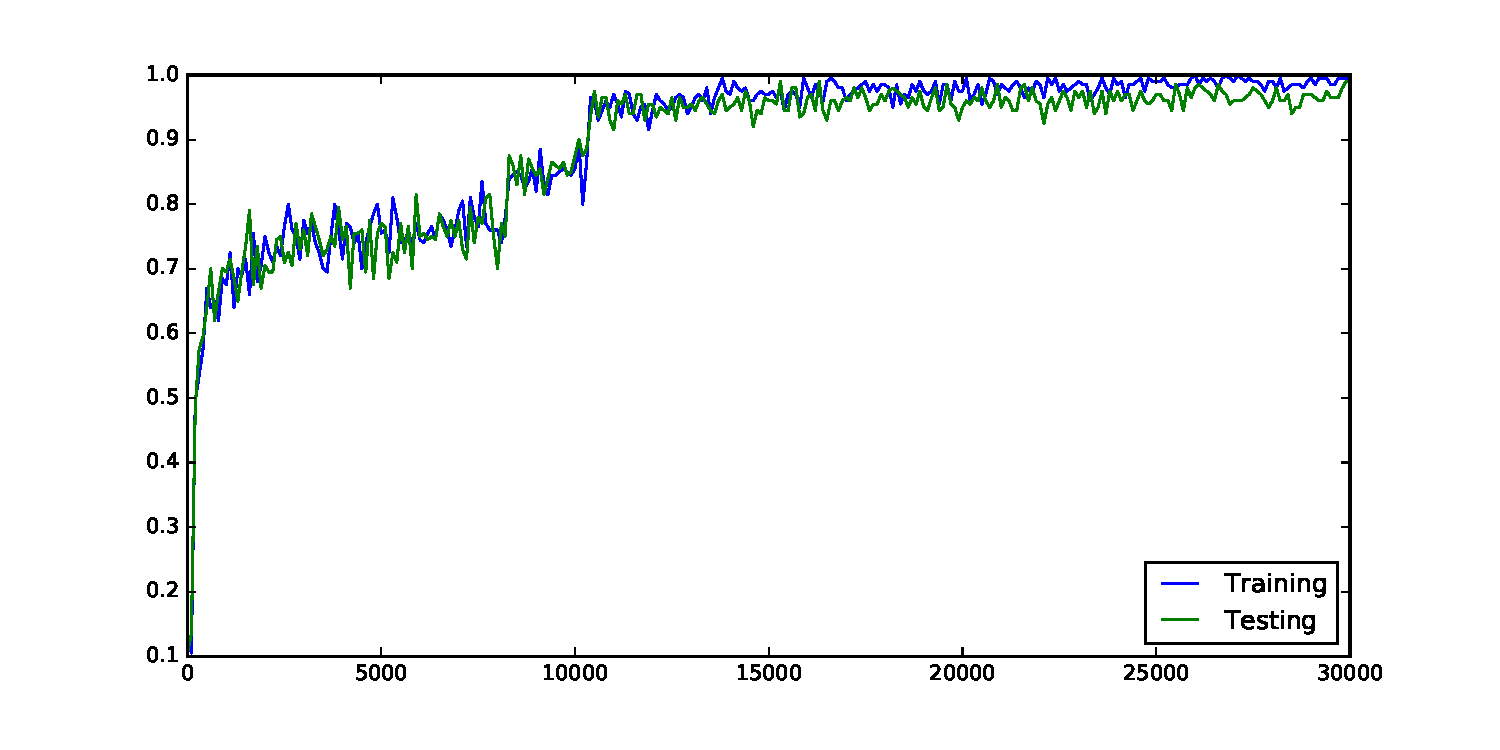
\includegraphics[width=\textwidth]{img/training_curve.pdf}
    \caption{Test and Train Accuracy through epochs. Final Test Accuracy: 96.9\%}
    \label{fig:training_curve}
\end{figure}

In a second time, once the principles of our implementation were validated by the first experiment, we have reimplemented our architecture using the two faster operations of Chebyshev Approximated Filters, and 1-D Max Pooling. Using this implementation allowed us to reach similar performance but in much shorter time as we can see on table \ref{tab:slow_fast}.

\begin{table}[]
    \centering
    \begin{tabular}{|l|c|}
        \hline
         Implementation & Epoch duration \\ \hline
         Graph Fourier Transform \& Transfert Matrix Pooling & 0.29s \\
         Chebyshev Approximation \& 1-D Max Pooling & 0.10s \\ \hline
    \end{tabular}
    \\
    \caption{Training epoch duration using slow and fast implementations, on GTX1080. The fast implementation allows a speedup of $\sim \times 3$.}
    \label{tab:slow_fast}
\end{table}


\subsection{Going Further with Autoencoding}

To push further the experiments already made in the paper, and to meet the final goal of this project, we have implemented a simple single filter autoencoder architecture, that we have trained in an unsupervised manner over the MNIST data. For the encoding part, we used the following Graph Convolutional stack:
\begin{itemize}
    \item Perform Graphical Filtering with largest Laplacian power $K_i=5$, and number of filters $n_i=1$
    \item Perform a ReLu Non-Linearity
    \item Perform a single Max Pooling to reduce the overall size about a factor $\sim 2$.
\end{itemize}
Concerning the decoder part, the data needs to be projected back to the larger graph at each stack. This is performed by simply projecting the signal values at coarsened nodes on their non-coarsened parents. This operation was easily implemented using the Transition matrix. Our Decoding Graph Convolutional stack was thus made of the following operations: 
\begin{itemize}
    \item Perform 2 Max UnPooling to enlarge the data of $\sim 2$
    \item Perform a ReLu Non-Linearity
    \item Perform a Graphical filtering with largest Laplacian power $K_i=5$, and number of filters $n_i=1$.
\end{itemize}

The overall architecture is composed of four Encoding Graph Convolutional stacks , and four Decoding Graph Convolutional stacks as depicted on figure \ref{fig:autoencoder}. We note that the embedded code is a vector of length $\sim60$ depending on the coarsening operation (compared to the input size $784$). 

\begin{figure}
    \centering 
    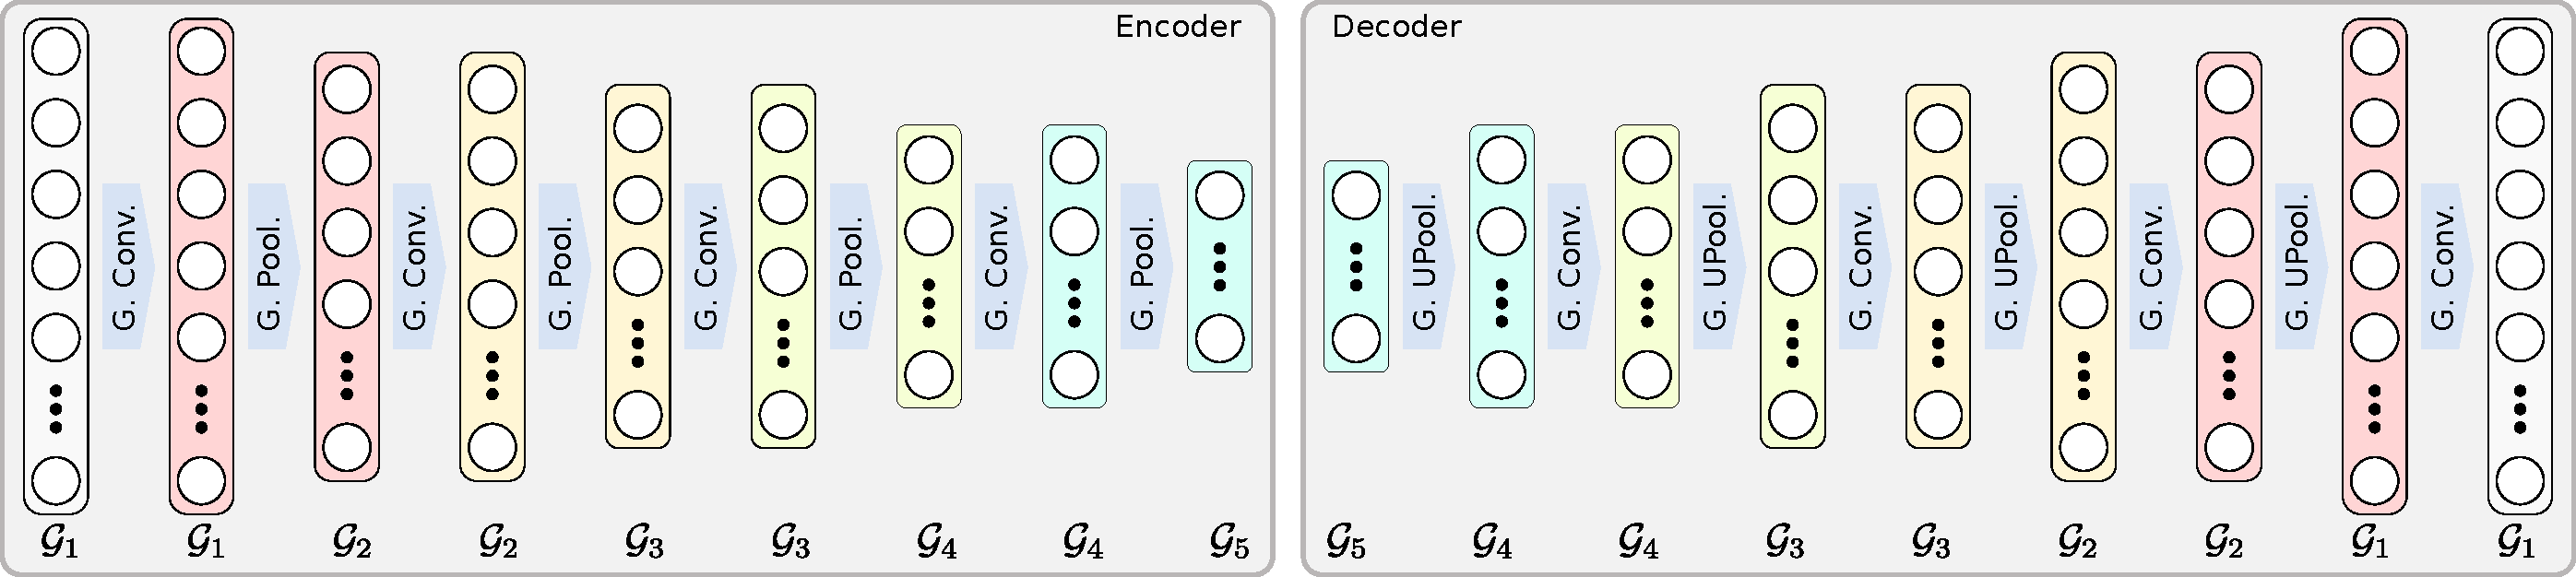
\includegraphics[width=\textwidth]{img/autoencoder.pdf}
    \caption{The architecture used to autoencode the MNIST DataSet, with signal structure.}
    \label{fig:autoencoder}
\end{figure}

We trained this architecture using a regularized L2-Distance:
\begin{equation}
    \mathcal{L}(x,\theta) = \|x-f(x)\|_2 + \alpha \sum_{j=1}^m \|\theta_j\|^2
\end{equation}
With $f(x)$, the output of the network for the training sample $x$. We trained the whole architecture from scratch, using again the AdaDelta Optimizer.

Using our trained autoencoder we were able to partially reconstruct samples as depicted on figure \ref{fig:reconstruction}. While keeping the overall shape of the digit, the reconstructions are still quite blurry, and our experiments have shown that the deeper the encoding, the blurrier the reconstruction was. To get deeper understanding of the learned embedded structure, we decoded some variable indicators of the embedded code (decode a $[0,0,1,0,0,\dots,0]$-like vector). When looking at the decoded plots of the first 16 indicators, we can see that the autoencoder has basically learnt to project the code signal from coarsened graph nodes to its parents nodes on the output space. In other words, it has learnt to approximate the identity operation. To our knowledge, it is a common pitfall in autoencoders, which can be overtaken using more complex forms of training (denoising for example). 

\begin{figure}
    \centering
    \subfigure[Reconstructed samples]{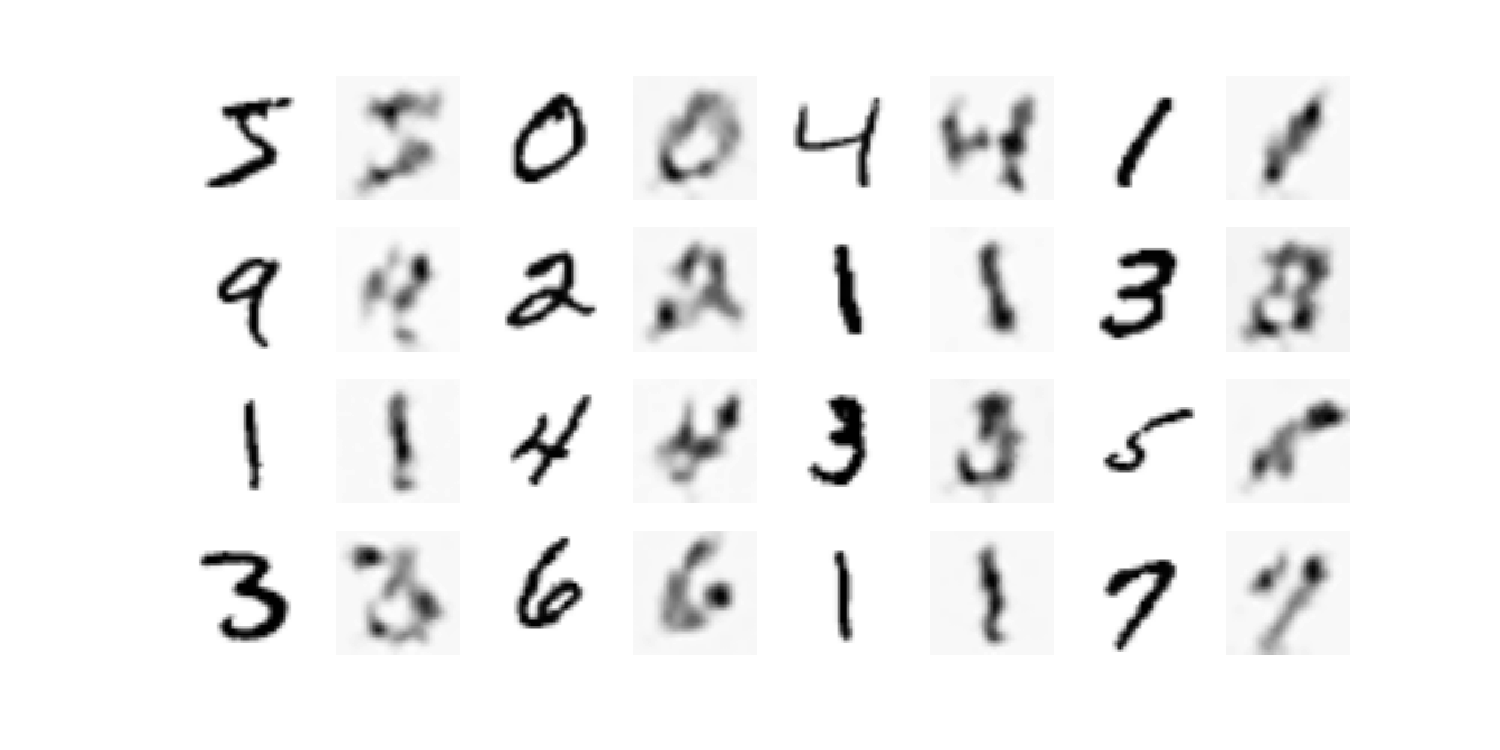
\includegraphics[width=0.66\textwidth]{img/reconstruction.pdf}}
    \subfigure[Code projection to output space]{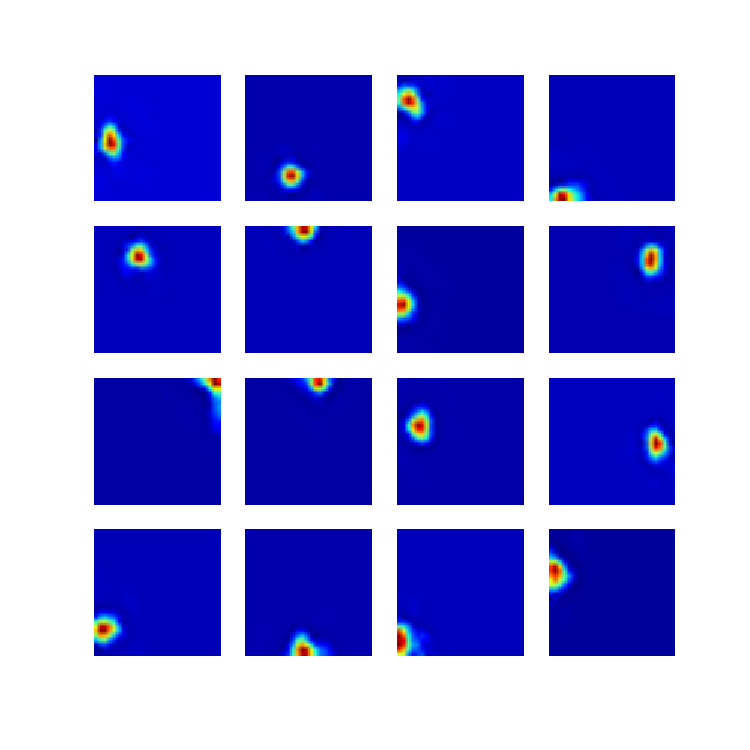
\includegraphics[width=0.33\textwidth]{img/code.pdf}}
    \caption{Reconstructed samples, and code variables projected to the output space}
    \label{fig:reconstruction}
\end{figure}

By the end of our experiments with autoencoders, it was still unclear if better behavior could be obtained using GCNN models. Once again, further work might be necessary to gain intuition about the potential of GCNN for autoencoding.